\documentclass[12pt,oneside]{book}
\usepackage{geometry}                		% See geometry.pdf to learn the layout options. There are lots.
\geometry{a4paper}                   			% ... or a4paper or a5paper or ... 
%\geometry{landscape}                		% Activate for for rotated page geometry
%\usepackage[parfill]{parskip}    		% Activate to begin paragraphs with an empty line rather than an indent
\usepackage{graphicx}				% Use pdf, png, jpg, or epsß with pdflatex; use eps in DVI mode
								% TeX will automatically convert eps --> pdf in pdflatex		
\usepackage{amssymb}

\usepackage[spanish]{babel}			% Permite que partes automáticas del documento aparezcan en castellano.
\usepackage[utf8]{inputenc}			% Permite escribir tildes y otros caracteres directamente en el .tex
\usepackage[T1]{fontenc}				% Asegura que el documento resultante use caracteres de una fuente apropiada.

\usepackage{hyperref}				% Permite poner urls y links dentro del documento

\title{Mi Juego Favorito}
\author{Javier Tibau}
%\date{}							% Activate to display a given date or no date

\begin{document}
\maketitle
\tableofcontents

\chapter{Introducción}
El libro a continuación es creado como una herramienta para el desarrollo de habilidades de edición colaborativa de documentos de texto plano. La herramienta que habilita dicha colaboración, en este taller, es Git pero podría ser reemplazada por otros sistemas de versionamiento.

\chapter{Los Juegos}

\section{Buscaminas}

\begin{figure}[htbp]
\begin{center}
\includegraphics[width=.60\textwidth]{./imagenes/minesweeper.png}
\caption{Buscaminas}
\label{Buscaminas}
\end{center}
\end{figure}
Buscaminas\footnote{\url{http://minesweeperonline.com/}} es uno de los juegos más jugados debido a lo ubicuo de su distribución. Fue incluido en 1992 en la versión de Windows 3.1 y desde entonces lo hemos encontrado presente en todas las versiones de dicho sistema operativo.
En la figura \ref{Buscaminas} puede ver una implementación web del juego.
La premisa del juego es simple: Limpiar el campo de juego sin hacer explotar ninguna de las minas que se encuentran en la cuadrícula.

\subsubsection{¿Por qué es uno de mis juegos favoritos?}
\begin{itemize}
\item[Javier Tibau] Las reglas del juego son sencillas y fáciles de entender. A pesar de esto, el juego no es atractivo para todo el mundo, creo que es un gusto adquirido. Las reglas me fueron presentadas por mi papá, quien en su máquina de trabajo con Windows 3.11 era uno de los pocos juegos ``divertidos'' que tenía. Para mi, el gran interés del juego es que destaca (o esconde) la resolución de problemas con fondo algebraico. En cierto momento del juego, y para el jugador que ha estudiado álgebra lineal, el reventar una casilla se torna similar a descifrar un sistema de ecuaciones con varias incógnitas. Los sistemas sencillos son bien definidos y tienen 2, 3 o hasta 4 incógnitas, mientras los más complejos pueden inclusive tener múltiples soluciones.
\end{itemize}

\section{Dota 2}

\begin{figure}[htbp]
\begin{center}
\includegraphics[width=.60\textwidth]{./imagenes/dota2.jpg}
\caption{Dota 2}
\label{Dota 2}
\end{center}
\end{figure}
Dota 2 \footnote{\url{http://dota2.com/}} es un juego creado por Valve basado en el popular mod de Warcraft 3, Defense of the Ancients. Es un juego de estrategia en equipo para ser jugado con equipos de 5 personas cada uno.
Dota 2 combina elementos de estrategia en tiempo real con perspectiva "en tercera persona", incorporando a todo ello un sistema de nivelación y jugabilidad de diversos juegos de rol como Diablo. Los jugadores asumen el papel de una unidad clasificado como un "héroe", que puede subir de nivel hasta un máximo de 25. La configuración básica de Dota 2 consiste en dos ciudades de distinta forma, cada una cuenta con una fortaleza de defensa conocida como "ancestro", situadas en los extremos opuestos de un mapa equilibrado de manera uniforme. Entre ellas hay varias regiones de conexión identificado como "caminos", que son atravesados por unidades enemigas, al tiempo que luchan contra poderosas torres defensivas a lo largo del camino. Los jugadores se dividen entre dos equipos, cada uno con hasta cinco jugadores, para competir como los principales defensores de cada Fortaleza de los Ancestros.

\subsubsection{¿Por qué es uno de mis juegos favoritos?}
\begin{itemize}
\item[Victor Cedeño] Este es un juego que requiere de comunicación y cooperación entre 5 personas para poder lograr el objetivo de vencer al otro equipo. Es muy dificil jugar solo sin la ayuda de tus compañeros. El juego tiene una gran selección de más de 100 heroes para elegir, esto quiere decir que cada partida es diferente ya que las combinaciones posibles de los equipos son innumerables. Es un juego que fomenta el trabajo en equipo y las decisiones correctas.
\end{itemize}

\include{juegos/Zelda}
\section{Twisted Metal: }

\begin{figure}[htbp]
\begin{center}
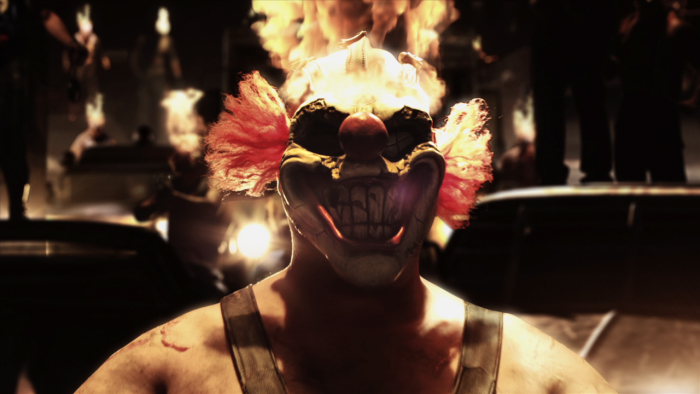
\includegraphics[width=.60\textwidth]{./imagenes/twistedmetal.jpg}
\caption{Twisted Metal}
\end{center}
\end{figure}

Twisted Metal es la primera entrega de la serie Twisted Metal. La historia del juego está centrada en el titular de la competencia en la que varios conductores de vehículos modificados deben destruir los otros vehículos en un intento por ser el último vivo. El ganador se reúne con el organizador de la competición, un misterioso hombre llamado Calypso, que otorgará al ganador un único deseo, independientemente de su precio, tamaño, o incluso de la realidad.
Twisted Metal recibió críticas dispares de la prensa especializada, pero el juego fue un éxito comercial, vendiendo más de 1.800.000 copias en los Estados Unidos.
\subsubsection{¿Por qué es uno de mis juegos favoritos?}
\begin{itemize}
\item[Juan Romero ] Twisted Metal es una de mis franquicias de juegos favoritos. He sido  fan desde hace mucho tiempo y comenzé a jugar la serie con Twisted Metal 3 para la consola de PlayStation 1 . Lo que me gustó de la experiencia fue que se combinan de forma única los juegos de conducción con los de  shooter en primera persona. Matar a los oponentes y ver como volaban en mil pedasos era lo que mas me divertia, ademas el hecho de que habia que tener buenas habilidades para manejar un vehículo,matar y estar pendiente de eludir los ataques de los demas contrincantes.
\end{itemize}
\section{Mortal Kombat Armageddon}

\begin{figure}[htbp]
\begin{center}
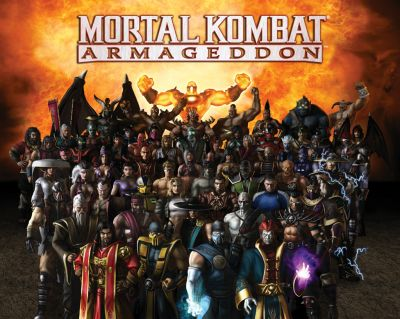
\includegraphics[width=.60\textwidth]{./imagenes/MortalK.jpg}
\caption{Mortal Kombat Armageddon}
\label{Mortal Kombat Armageddon}
\end{center}
\end{figure}

Mortal Kombat: Armageddon \footnote{\url{http://www.mortalkombat.net/armageddon/}} es un videojuego de la saga Mortal Kombat desarrollada por Midway Games. Este juego es una continuación directa de Mortal Kombat: Deception. El juego distribuyo más de 2 millones de copias por todo el mundo.
Las plataformas designadas para este juego son PlayStation 2 y Xbox en el 2006 y Wii en el 2007.

\subsubsection{¿Por qué es uno de mis juegos favoritos?}
\begin{itemize}
\item[Joao Sanga] Me gusta mucho por los gráficos, el modo de pelea y la historia. Las peleas en Mortal Kombat siempre conservarán su puntito gore (sangriento): sin él, nada diferenciaría a la saga de otros tantos juegos de lucha.
Aprendiendo de la experiencia en títulos pasados, MK Armageddon ha suavizado los controles, y ha ordenado todos los elementos en un sencillo menú. Pero la mecánica del juego sigue siendo la misma: cada luchador tiene dos métodos de combate –una técnica cuerpo a cuerpo, y lucha con arma-, junto con los clásicos combos aéreos, encadenados, llaves y contras. Quienes busquen un título de machaque fácil pulsando botones a toda velocidad, lo tienen complicado de nuevo: en Mortal Kombat los combates no lo parecen, SON lentos, ni de lejos tan vertiginosos como en cualquier juego de lucha de Namco. Los kombatientes se mueven en ocasiones como marionetas que responden mecánicamente a nuestras teclas.
En conclusión, Mortal Kombat Armageddon es uno de los mejores creados de la saga de Mortal Kombat.
\end{itemize}


\chapter{Conclusiones}
Cuales juegos fueron más populares y un breve razonamiento del porqué.

\end{document}  
